%%%%%%%%%%%%%%%%%%%%%%%%%%%%%%%%%%%%%%%%%
% Beamer Presentation
% LaTeX Template
% Version 1.0 (10/11/12)
%
% This template has been downloaded from:
% http://www.LaTeXTemplates.com
%
% License:
% CC BY-NC-SA 3.0 (http://creativecommons.org/licenses/by-nc-sa/3.0/)
%
%%%%%%%%%%%%%%%%%%%%%%%%%%%%%%%%%%%%%%%%%

%----------------------------------------------------------------------------------------
%	PACKAGES AND THEMES
%----------------------------------------------------------------------------------------

\documentclass{beamer}

\mode<presentation> {

% The Beamer class comes with a number of default slide themes
% which change the colors and layouts of slides. Below this is a list
% of all the themes, uncomment each in turn to see what they look like.

%\usetheme{default}
%\usetheme{AnnArbor}
%\usetheme{Antibes}
%\usetheme{Bergen}
%\usetheme{Berkeley}
%\usetheme{Berlin}
\usetheme{Boadilla}
%\usetheme{CambridgeUS}
%\usetheme{Copenhagen}
%\usetheme{Darmstadt}
%\usetheme{Dresden}
%\usetheme{Frankfurt}
%\usetheme{Goettingen}
%\usetheme{Hannover}
%\usetheme{Ilmenau}
%\usetheme{JuanLesPins}
%\usetheme{Luebeck}
%\usetheme{Madrid}
%\usetheme{Malmoe}
%\usetheme{Marburg}
%\usetheme{Montpellier}
%\usetheme{PaloAlto}
%\usetheme{Pittsburgh}
%\usetheme{Rochester}
%\usetheme{Singapore}
%\usetheme{Szeged}
%\usetheme{Warsaw}

% As well as themes, the Beamer class has a number of color themes
% for any slide theme. Uncomment each of these in turn to see how it
% changes the colors of your current slide theme.

%\usecolortheme{albatross}
\usecolortheme{beaver}
%\usecolortheme{beetle}
%\usecolortheme{crane}
%\usecolortheme{dolphin}
%\usecolortheme{dove}
%\usecolortheme{fly}
%\usecolortheme{lily}
%\usecolortheme{orchid}
%\usecolortheme{rose}
%\usecolortheme{seagull}
%\usecolortheme{seahorse}
%\usecolortheme{whale}
%\usecolortheme{wolverine}

%\setbeamertemplate{footline} % To remove the footer line in all slides uncomment this line
%\setbeamertemplate{footline}[page number] % To replace the footer line in all slides with a simple slide count uncomment this line

%\setbeamertemplate{navigation symbols}{} % To remove the navigation symbols from the bottom of all slides uncomment this line
}
\usepackage{float}
\usepackage{macro}
\usepackage{graphicx} % Allows including images
\usepackage{booktabs} % Allows the use of \toprule, \midrule and \bottomrule in tables
\usepackage[french]{datetime}
\usepackage[utf8]{inputenc}
\usepackage{tabularx}
\usepackage{algorithm,algorithmic}
\usepackage{xcolor}
\usepackage{tikz}
\usepackage{listings}
\usetikzlibrary{positioning,fit,calc}
\usepackage{xspace}
\usepackage{color}
\usepackage{colortbl}
\usepackage{array}
%----------------------------------------------------------------------------------------
%	TITLE PAGE
%----------------------------------------------------------------------------------------

\title[Micromouse]{Véhicule autonome Micromouse} % The short title appears at the bottom of every slide, the full title is only on the title page

\author[]{
    Djahid ABDELMOUMENE \break
    Amine AGRANE \break
    Ishak AYAD \break
    Donald LAY 
} % Your name
 
\titlegraphic{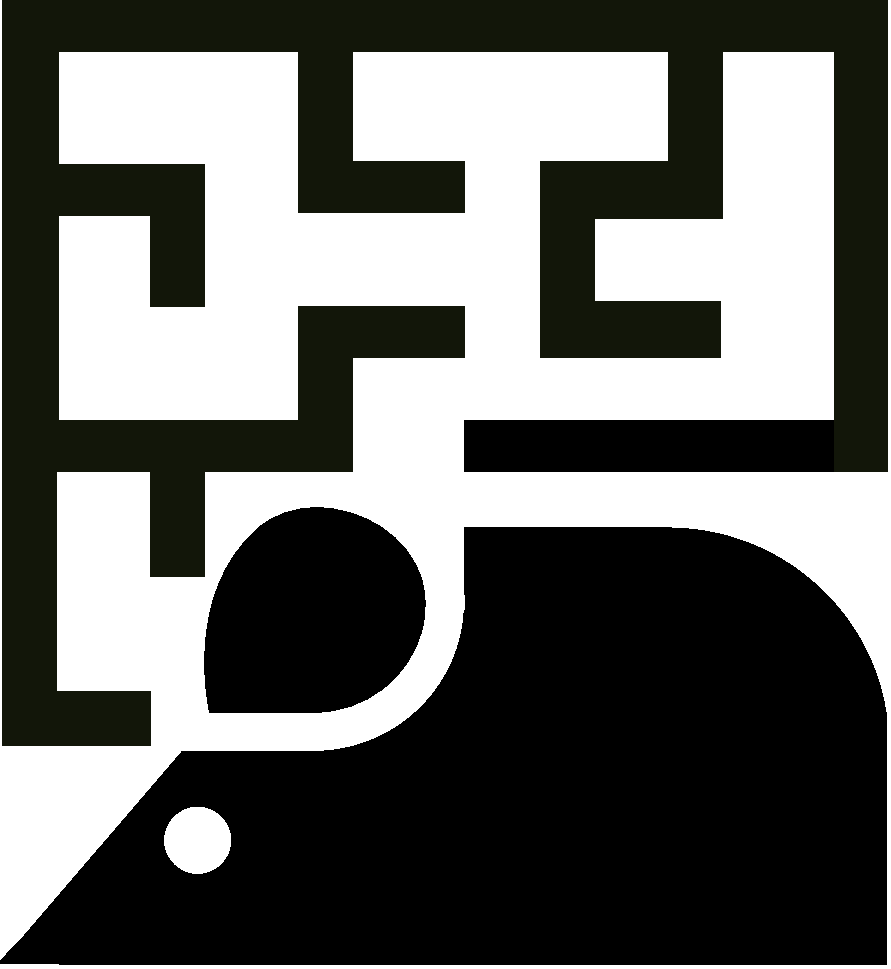
\includegraphics[width=0.9cm]{pics/MMLogo.pdf}% \hspace*{1cm}~
% 
\includegraphics[height=0.7cm]{pics/cyulogo.png}
}

% \logo{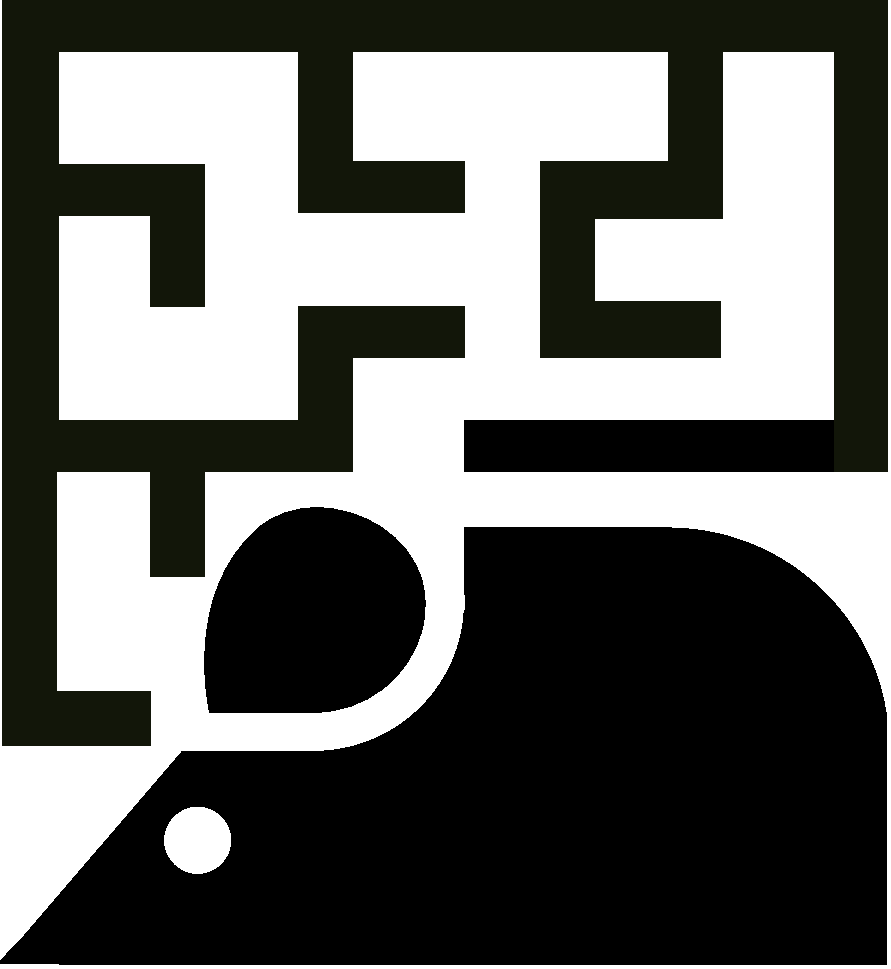
\includegraphics[scale=0.03]{pics/MMLogo.pdf}} % add the project logo

\institute[CYU] % Your institution as it will appear on the bottom of every slide, may be shorthand to save space
{
Tuteur technique: M. Alexandre PITTI \\
Encadrant de gestion de projet: M. Tianxiao LIU \\
\medskip
Master IISC - UE Projet de Synthèse \\
\medskip
CY Cergy-Paris Université % Your institution for the title page
\medskip

%\textit{} % Your email address
}
\date{24 avril 2020} % Date, can be changed to a custom date

\begin{document}

\begin{frame}
\titlepage % Print the title page as the first slide
\end{frame}

\begin{frame}
\frametitle{Table des matières} % Table of contents slide, comment this block out to remove it
\tableofcontents[]  % Throughout your presentation, if you choose to use \section{} and \subsection{} commands, these will automatically be printed on this slide as an overview of your presentation
\end{frame}

%----------------------------------------------------------------------------------------
%	LES SLIDES DE PRESENTATION 15 à 17 slides
%----------------------------------------------------------------------------------------

% Introduction de projet environ 2 slides
\section{Introduction}

\subsection{Objectifs du projet}
\begin{frame}{Objectifs du projet}
Réaliser un véhicule autonome pour la résolution d'un labyrinthe. 

\vspace{5mm}

\begin{center}
    
\begin{table}[H]
\scalebox{0.9}{
    \begin{tabular}{|l|l|l|}
        \toprule
        \textbf{Simulation} & \textbf{Brain} & \textbf{Communication}\\
        \midrule
            Simulation des capteurs & 
            Estimation de position & 
            Définition de protocole \\
            \hline
            
            Génération de maze & 
            Contrôle de véhicule &
            Comm. inter-process\\
            \hline
            
            Simulation des collisions & 
            Algorithme de navigation &
            Bus entre machines\\
            
        \bottomrule
    \end{tabular}
}
    \caption{Objectifs à réaliser pour les trois parties essentielles}
\end{table}

\end{center}
% En plus de la résolution du labyrinthe des systèmes Multi-Agent, \textit{i.e.} des jeux avec plusieurs véhicules seront mis en oeuvre.

%En plus de la résolution du labyrinthe, des jeux avec plusieurs véhicules seront mis en oeuvre.

Réaliser des jeux compétitifs et coopératifs entre plusieurs véhicules.
\end{frame}

\subsection{Mise en scénario}
\begin{frame}{Mise en scénario}

\begin{center}
    
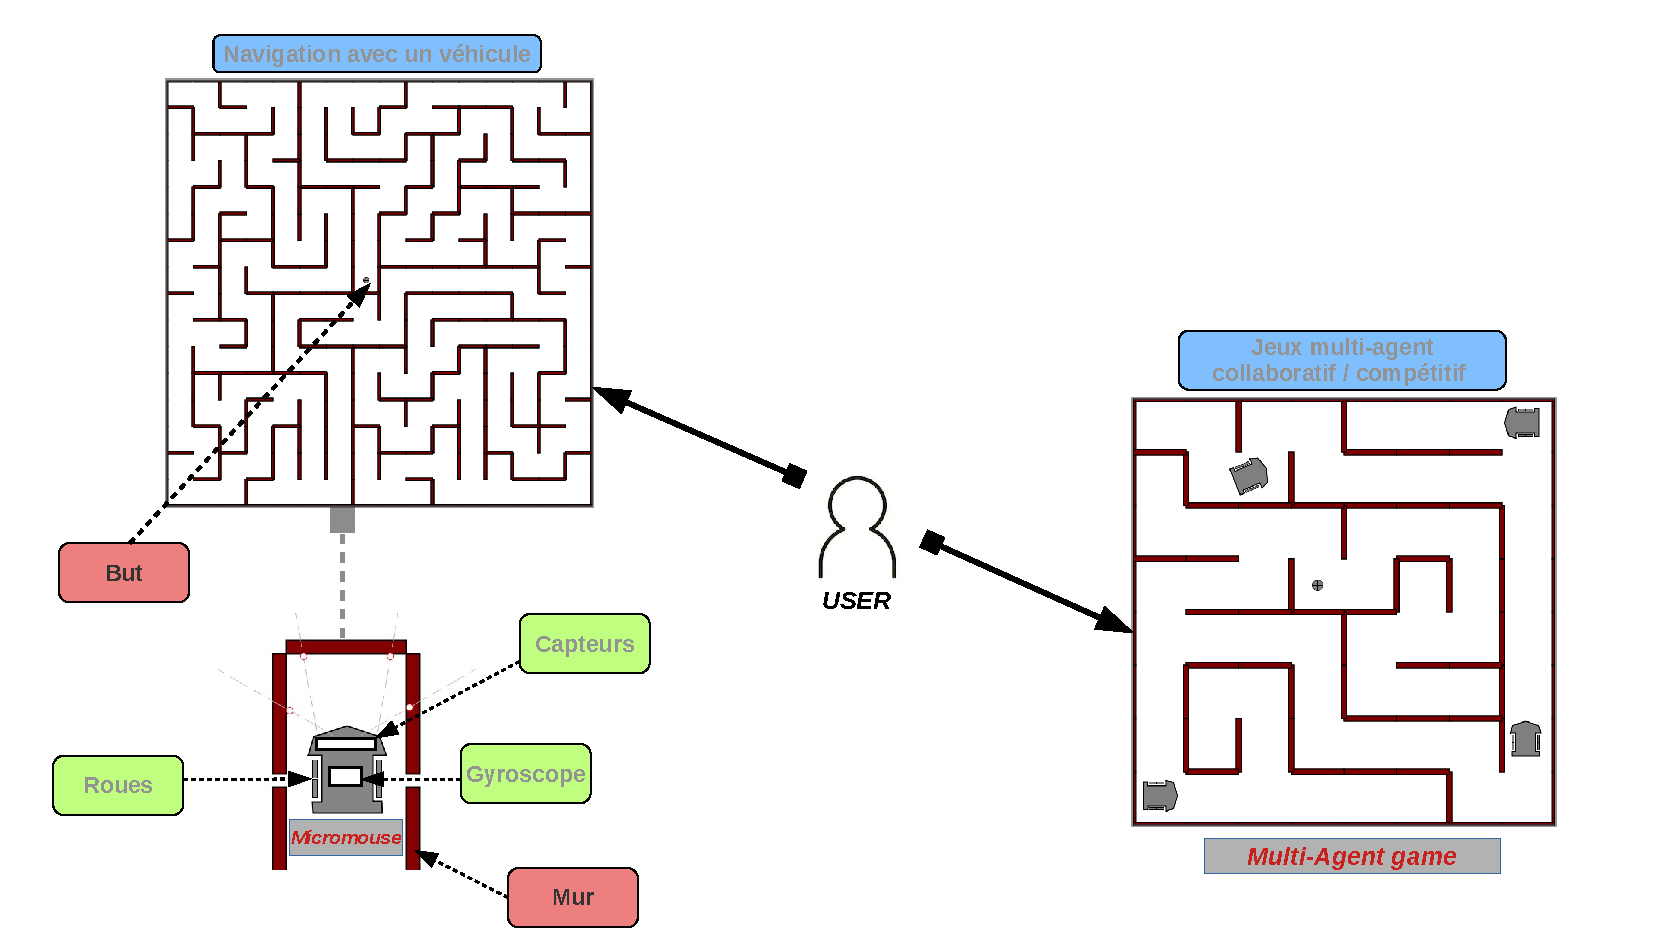
\includegraphics[width=12cm,height=7cm,keepaspectratio]{pics/mise_en_scenario.pdf}

\end{center}
\end{frame}


% Fin Contexte du Introduction

% Partie technique de projet, environ 10 slides

\begin{frame}{Architecture technique globale}
L'architecture des différents parties techniques de projet.

\begin{center}

\begin{table}[H]
    \setlength{\tabcolsep}{12pt}
    \begin{tabular}{l l}
        \toprule
        \textbf{Simulation} & \textbf{Brain} \\
        \midrule
            Simulation des capteurs & 
            Estimation de position  \\
            \hline
        
            Module communication & 
            Module communication \\
            \hline
            
            Génération de maze & 
            Contrôle de véhicule \\
            \hline
            
            Simulation des collisions & 
            Algorithme de navigation \\
        
        \bottomrule
    \end{tabular}
    \caption{Composants des différents modules du système.}
\end{table}

\tikzstyle{block} = [rectangle, draw, fill=blue!10, rounded corners, text centered,     text width = 7em, minimum height = 2em]


\begin{tikzpicture}[remember picture,
  inner/.style={scale=0.8,block, align=left,draw=blue!50,fill=blue!20,thick,inner sep=3pt},
  outer/.style={scale=0.8,draw=green,fill=green!20,thick,inner sep=10pt}
  ]
  \node[outer,label=Simulation] (A) {
    \begin{tikzpicture}
      \node [inner,draw=blue] (col) {Simulation \\de collisions};
      \node [inner,draw=blue,above=of col] (acom)  {Module \\communication};
      \node [inner,draw=blue,left=of acom] (cap)  {Simulation \\de capteurs};
      \node [inner,draw=blue,left=of col] (maze) {Génération \\de maze};
      
      \draw[black,thick,->] (maze) -- (col);
      \draw[black,thick,->] (col) -- (cap);
      \draw[black,thick,->] (acom) -- (col);
      \draw[black,thick,->] (cap) -- (acom);
    \end{tikzpicture}
  };
  \node[outer,right=1.5cm of A,label=Brain] (B) {
    \begin{tikzpicture}
      \node [inner,draw=blue] (pos)  {Estimation \\de position};
      \node [inner,draw=blue, below=of pos] (nav) {Algorithme \\de navigation};
      \node [inner,draw=blue, left=of pos] (bcom)  {Module \\communication};
      \node [inner,draw=blue, left=of nav] (ctrl) {Contrôle \\de véhicule};

      \draw[black,thick,->] (pos) -- (nav);
      \draw[black,thick,->] (nav) -- (ctrl);
      \draw[black,thick,->] (ctrl) -- (bcom);
      \draw[black,thick,->] (bcom) -- (pos);
      

    \end{tikzpicture}
  };

  \draw[black,thick,->] (A.-365) -- node[scale=0.8,below] {Capteurs} (B.-535);
  \draw[black,thick,->] (B.535) -- node[scale=0.8,above] {Moteurs} (A.365);
\end{tikzpicture}
\end{center}

\end{frame}

\section{Simulation}

\subsection{Modèle physique de Micromouse}
\begin{frame}{Modèle physique de Micromouse}
Le véhicule est modélisé comme un polygone 2D, avec les quatre roues placées sur les côtés du véhicule, avec les propriétés suivantes:
\begin{columns}[c]
\column{.45\textwidth}
\begin{itemize}
    \item Pas de force de gravité
    \item Force de traînée sur le corps et les roues
    \item Force de frottement
    \item Résistance latérale des roues
    \item Résistance angulaire des roues
\end{itemize}

\column{.55\textwidth} % Left column and width
\fig{pics/wheelForces.png}{8cm}{5cm}{Forces appliquées sur les roues.}{wheelF}

\end{columns}
\end{frame}

\subsection{Simulation de capteurs distance}
\begin{frame}{Simulation de capteurs distance}
Les capteurs de distance sont modélisés comme des Raycasts à partir des positions et orientations des capteurs réels sur le corps de la Micromouse.
\fig{pics/dist_sensor.png}{8cm}{5cm}{Les capteurs de distances dans la simulation. Chaque raycast (ligne pointillée) représente un capteur et sa projection sur les murs (cercle rouge)}{distsensor}

\end{frame}

\subsection{Simulation de l'accéléromètre et gyroscope}
\begin{frame}{Simulation de l'accéléromètre et gyroscope}

Un autre type de capteur (accéléromètre et gyroscope) est utilisé pour détecter l'accélération directionelle et angulaire du véhicule. \\


\vspace{5mm}
La simulation de celle-ci se fait avec la méthode d'intégration de Verlet (équation ci-dessous), en utilisant des échantillons des valeurs de position et de direction de la Micromouse : \\
\begin{equation*}
    \vec{a}_n = \frac{\vec{x}_{n+1} - 2 * \vec{x}_n + \vec{x}_{n-1}}{\Delta t^2}
\end{equation*}\\
Cette méthode donne un facteur d'erreur quadratique sur la valeur d'accélération $\mathcal{O}(\Delta t^2)$ à chaque itération.
\end{frame}

\subsection{Algorithmes de génération de labyrinthe}


\begin{frame}{Algorithmes génération de labyrinthe}
\begin{itemize}
\item Les labyrinthes peuvent être classifiés en deux types :   parfaits et imparfaits.
\item On utilise différents algorithmes de génération de labyrinthes : algorithme de Backtracking, Kruskal, etc.

\fig{pics/maze.png}{6cm}{5cm}{Génération d'un labyrinthe à l'aide de l'algorithme de Backtracking.}{genmaze}
\end{itemize}
\end{frame}

%------------------------------- BEGIN section brain

\section{Brain}
\begin{frame}{Contrôle et navigation de la micromouse (Brain)}

\fig{pics/brain_process.png}{12.5cm}{6.7cm}{Éléments importants du brain et leurs interactions.}{brainProcess}

\end{frame}

\subsection{Estimation de la pose}
\begin{frame}{Estimation de la pose}

%Une des parties les plus importantes du Brain est l'estimation de la position et de l'orientation de véhicule, en utilisant les capteurs d'accélération.
Une des parties permettant le contrôle de véhicule est l'estimation de la position et orientation, qui utilise les capteurs d'accélération.

\begin{figure}
\centering
\tikzstyle{block} = [rectangle, draw, fill=blue!10,rounded corners,  text centered,     text width = 7em, minimum height = 2em]
\begin{tikzpicture}[remember picture,
  inner/.style={block, text centered, scale=0.78,align=left,draw=blue!50,fill=blue!20,thick,inner sep=3pt},
  txtedge/.style={scale=0.78,above,midway},
  operator/.style={scale=0.78,circle,draw, fill=blue!10, text centered},
  outer/.style={scale=0.78,draw=green,fill=green!20,thick,inner sep=10pt}
  ]
\node [inner] (ang) {Estimation \\de l'orientation};
\coordinate[left=2cm of ang] (lft);
\node [inner, below=of ang] (dep) {Estimation \\de déplacement};
\coordinate[left=2cm of dep] (lft2);
\node [operator, right=of dep] (rot) {rot.};
\node [operator, right=of rot] (plus) {+};


\coordinate [right=of plus] (pos);
\node [inner, below=of pos] (cur) {Position courant};
\node [inner, below=of cur] (init) {Position initiale};
\coordinate[right=2.5cm of pos] (rgt2);
\coordinate[right=2cm of pos] (rgt3);
\coordinate[above=1.8cm of rgt2] (rgt);
\coordinate[above=1.4cm of rot] (abvrot);
\node [inner, below=of cur] (init) {Position initiale};

\draw [->] (lft) -- (ang) node [txtedge] {Gyroscope};
\draw [->] (lft2) -- (dep) node [txtedge] {Accéléromètre};
\draw [->] (dep) -- (rot) node [txtedge] {$\Delta \vec{p}$};
\draw [] (abvrot) -- (rot);
\draw [->] (rot) -- (plus);
\draw [] (plus) -- (rgt3) node [txtedge] {$\vec{p}$};
\draw [->] (rgt3) |- (cur);
\draw [->] (cur) -| (plus);

\draw [] (ang) -- (abvrot)  node [txtedge] {$\theta$};
\draw [->] (abvrot) -- (rgt) node [txtedge] {L'angle estimé};
\draw [->] (rgt3) -- (rgt2);
\draw [->] (init) -- (cur) node [txtedge,rotate=90](intlbl) {init.};

\node [scale=0.8,thick,inner sep=25pt,draw=green, label=Estimation de postion, fit=(cur)(init)(plus)(pos)(intlbl)(rot)(rgt3)] (out) {};

\end{tikzpicture}
\caption{Diagramme de l'estimation de pose.} \label{fig:estimpos}
\end{figure}
\end{frame}  

\subsection{Algorithmes de navigation}
\begin{frame}{Algorithme de Flood fill}
Étant donné une matrice ($\mathrm{L}$), imaginez que vous versez de l'eau depuis $\mathcal{C}_a$.

\begin{columns}[c]

\column{.45\textwidth}
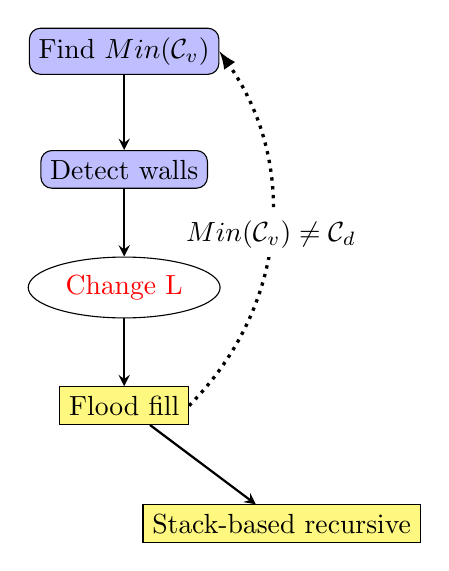
\begin{tikzpicture}
\usetikzlibrary{arrows}
\usetikzlibrary{shapes}

\tikzstyle{debutfin}=[ellipse, draw, text=red]
\tikzstyle{instruct}=[rectangle, draw, fill=yellow!50]
\tikzstyle{test}=[diamond, aspect=2.5, thick, draw=blue, fill=yellow!50, text=blue]
\tikzstyle{es}=[rectangle, draw, rounded corners=4pt, fill=blue!25]
\tikzstyle{suite}=[->, >=stealth, thick, rounded corners=4pt]
\tikzstyle{loop}=[->,>=latex,very thick,dotted]

%placement des nœuds
\node[es] (find) at (-7,8) {Find $Min(\mathcal{C}_v)$};
\node[es] (walls) at (-7,6.5) {Detect walls};
\node[debutfin] (change) at (-7,5) {Change $\mathrm{L}$};
\node[instruct] (flood) at (-7,3.5) {Flood fill};
\node[instruct] (recursive) at (-5,2) {Stack-based recursive};

%Placement des flèches
\draw[suite] (find) -- (walls);
\draw[suite] (walls) -- (change);
\draw[suite] (change) -- (flood);
\draw[suite] (flood) -- (recursive);
\draw[loop] (flood.east) to [bend right=40] node[midway,fill=white] {$Min(\mathcal{C}_v) \neq \mathcal{C}_d$} (find.east);
\end{tikzpicture}

\column{.55\textwidth} % Left column and width
\fig{pics/flood_neighbours.png}{5cm}{5cm}{Dispersion de l'eau}{floodNeighbours}

\end{columns}

\end{frame}

\begin{frame}{Algorithme Q Learning apprentissage renforcé}
L'agent (Micromouse) reçoit une récompense (+, -) pour chaque déplacement.

\begin{columns}[c]

\column{.55\textwidth}

On note :
\begin{itemize}
    \item $\mathrm{s}$ un état et $\mathrm{a}$ une action.
    \item $\mathrm{r(.)}$ la récompense reçue en entrant dans un nouvel état.
    \item $\gamma$ le facteur d'actualisation.
    \item $\alpha$ le taux d'apprentissage.
\end{itemize}

\column{.45\textwidth}
\fig{pics/state_action_table.png}{5cm}{5cm}{Q-table}{Qtable}
\end{columns}

\begin{center}
\large{
$\mathcal{Q}(\mathrm{s},\mathrm{a}) = \mathcal{Q}(\mathrm{s},\mathrm{a}) + \alpha . (\mathrm{r}(\mathrm{s'}) + \gamma . max(\mathcal{Q}(\mathrm{s'},\mathrm{a'})) - \mathcal{Q}(\mathrm{s},\mathrm{a}))$}

\color{red}
Bellman Equation
\end{center}

\end{frame}

\begin{frame}{Algorithme RRT rapidly exploring random tree}

Plusieurs extensions de l'algorithme rapidly exploring random tree.

\begin{figure}
    \centering
    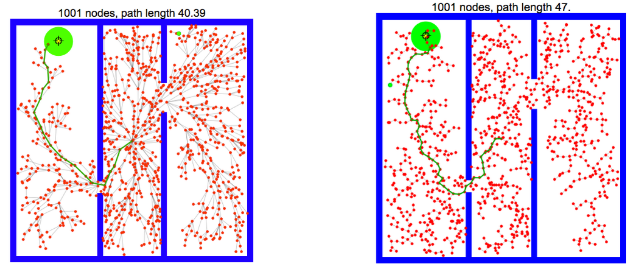
\includegraphics[width=11cm,height=10cm,keepaspectratio]{pics/rrt_rrtstar.png}
    \caption{Comparaison entre RRT* et RRT pour 1000 noeuds}
\end{figure}

RRT* ou Sampling-based Algorithms for Optimal Motion Planning, chaque fois qu'on ajoute un noeud on simplifie le chemin.

\end{frame}

%------------------------------- END section brain

\section{Communication}

\subsection{Modules de communication}
\begin{frame}{Modules de communication}

\fig{pics/comm_pipes_design.png}{12cm}{10cm}{Utilisation des named pipes pour la communication inter-processus }{commdiag}
\end{frame}

\subsection{Protocole de communication}
\begin{frame}{Protocole de communication}

\fig{pics/msg_format.jpg}{8cm}{5cm}{Format de message (en bits)}{msgfmt}

\begin{table}
    \begin{tabular}{ |l|l|l|l| }
        \toprule
        \textbf{Flag} & \textbf{Taille} & \textbf{Données} & \textbf{Description}\\
        \midrule
            10 & 
            17 octets & 
            7 int & 
            \begin{tabular}{@{}l@{}}
                - Dimension du labyrinthe \\
                - Position de départ et d'arrivée \\
            \end{tabular} \\
            \hline
        
            11 & 
            41 octets & 
            10 float & 
            \begin{tabular}{@{}l@{}}
                - Capteurs de distance \\
                - Accéléromètre \\
            \end{tabular} \\
            \hline
            
            20 & 
            9 octets & 
            2 float &
            \begin{tabular}{@{}l@{}}
                - Puissance des moteurs \\
            \end{tabular} \\
        \bottomrule
    \end{tabular}
    \caption{Types de messages du protocole de communication.}
\end{table}

\end{frame}
% Fin partie technique

% Avancement actuel de projet 1 à 2 slides
\section{Avancement actuel}
\begin{frame}{Avancement actuel}

\begin{center}

\begin{table}[H]
    \centering
    \begin{tabularx}{\textwidth}{>{\columncolor{green!15}}X >{\columncolor{red!15}}X}
        \toprule
            \textbf{Ce qui a été fait} & \textbf{Ce qui reste à faire} \\
        \midrule
            Simulation du véhicule & 
            Réalisation des algorithmes de contrôle\\ 
            \hline
            
            Génération de labyrinthe & 
            Amélioration/optimisation des algorithmes actuels \\ 
            \hline
            
            Implémentation de l'algorithme de Flood fill  &     
            Réalisation d'un système multi-agents\\
            \hline
            
            Communication Simulation/Brain & 
            Extension des algorithmes de navigation\\
            \hline

            Estimation de la pose &
            Génération de labyrinthes imparfaits \\
        \bottomrule
    \end{tabularx}
    \caption{Tableau de suivi d'avancement du projet.}
\end{table}

\end{center}

\end{frame}

%----------------------------------------------------------------------------------------

\end{document} 